\chapter{Analisis}
Bagian ini akan menganalisis perbedaan penggunaan \textit{framework} \textit{front-end} Foundation 6 dan Bootstrap 4. Dua hal yang dibahas adalah penggunaan sistem grid dan komponen - komponen untuk kedua \textit{framework} tersebut.
\section{Sistem Grid}
Sistem grid bertujuan untuk menentukan tata letak dalam situs web yang setiap grid dipisahkan oleh garis yang tak terlihat dimana elemen ditempatkan.  Sehingga struktur grid yang terbentuk menciptakan perataan yang efektif dan konsisten dalam desain. Sebuah grid tersusun dari kolom dan baris serta jarak antar baris dan kolom yang disebut gutter. \\
\noindent Kedua \textit{framework} menggunakan Flexbox yaitu metode layout untuk penataan item dalam suatu halaman dengan mengatur posisi dan keteraturan dalam suatu \textit{container}.\noindent Berikut ini gambar ~\ref{fig:nonflexbox} apabila tidak menggunakan flexbox:
\begin{figure} [H]
	\centering  
	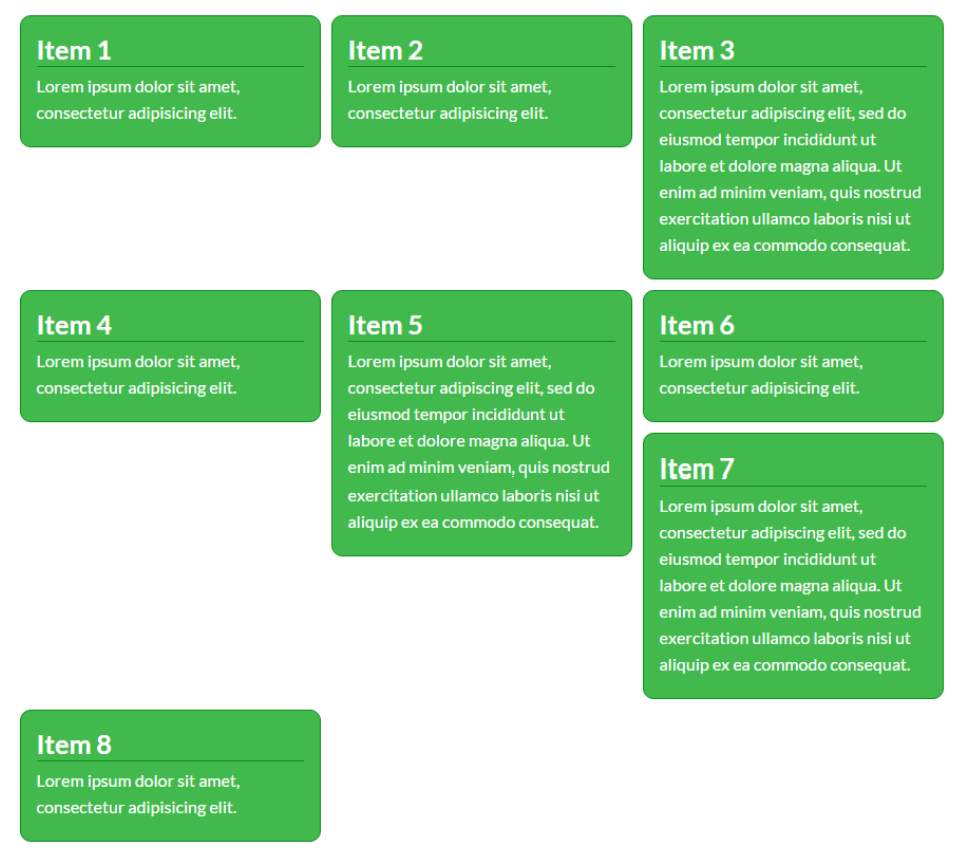
\includegraphics[scale=0.5]{analisis/nonflexbox_bootstrap.png}  
	\caption{Tanpa flexbox grid pada Bootstrap 4}
	\label{fig:nonflexbox}	 
\end{figure}
\noindent Lalu pada gambar ~\ref{fig:flexbox} apabila menggunakan flexbox grid maka setiap kolom akan disesuaikan tingginya. Sehingga dapat mengatur ukuran layout ketika diakses dalam device yang berbeda. Disini flexbox mampu memodifikasi lebar atau tinggi dari child item yang tersedia tanpa menggunakan floats.
\begin{figure} [H]
	\centering  
	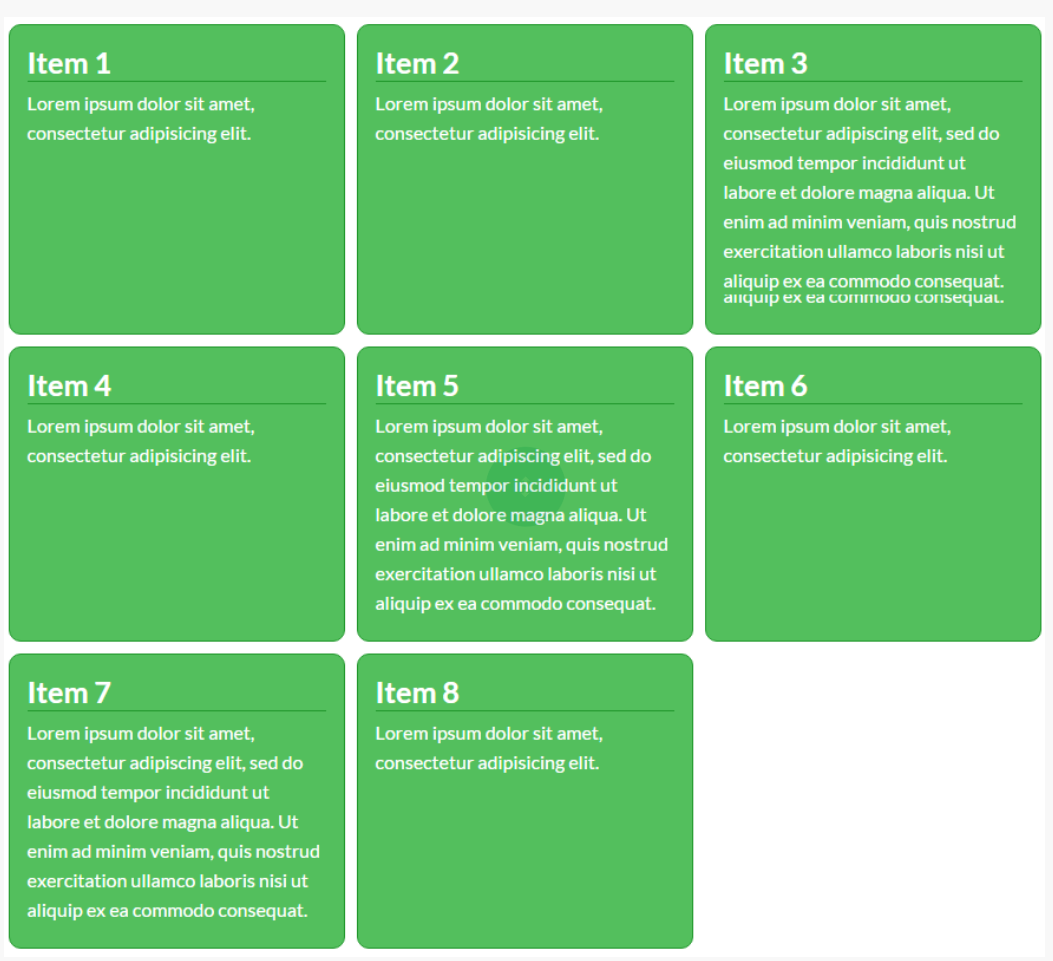
\includegraphics[scale=0.5]{analisis/flexbox_bootstrap.png}  
	\caption{Tanpa flexbox grid pada Bootstrap 4}
	\label{fig:flexbox}	 
\end{figure}
Berikut ini penjelesan mengenai perbedaan sistem grid pada Foundation 6 dan Bootstrap 4.
\subsubsection{Foundation 6: XY Grid}
XY grid merupakan grid \textit{default} dari foundation 6 yang mendukung banyak tipe grid yaitu grid margin, grid padding, grid blok dan grid vertikal. X menunjukkan arah horizontal dan Y menunjukkan arah vertikal.
Berikut ini beberapa fitur yang tersedia ketika menggunakan sistem XY grid:
\begin{figure} [H]
	\centering  
	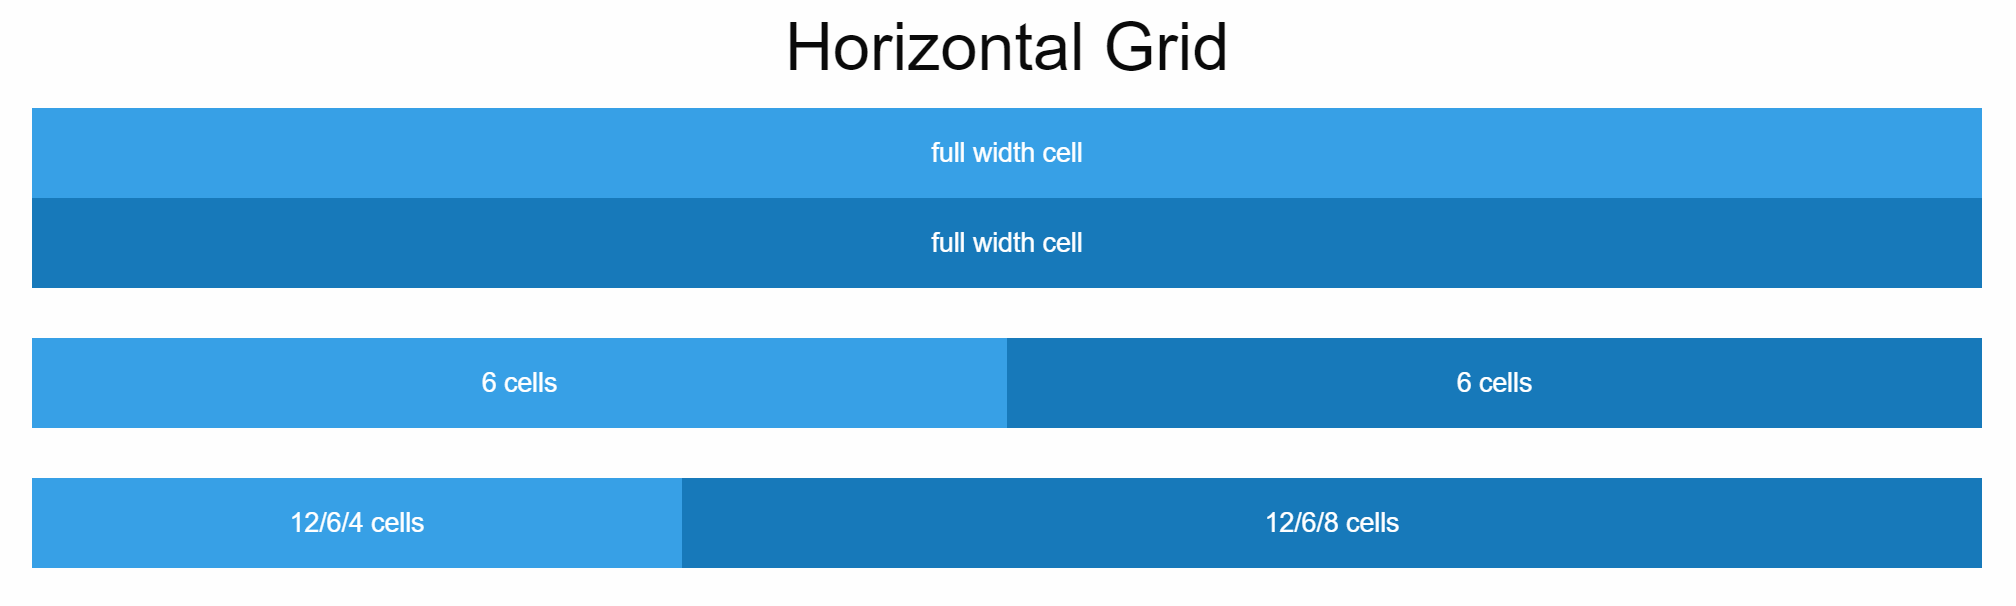
\includegraphics[width=\textwidth,height=\textheight,keepaspectratio]{analisis/grid1_f.png}
	\caption{Horizontal Grid  pada Foundation 6.}
	\label{fig:grid1f}
\end{figure}
Pada gambar ~\ref{fig:grid1f} kolom dapat disejajarkan dengan cara yang sama seperti menyelaraskan teks dalam paragraf.
\begin{figure} [H]
	\centering  
	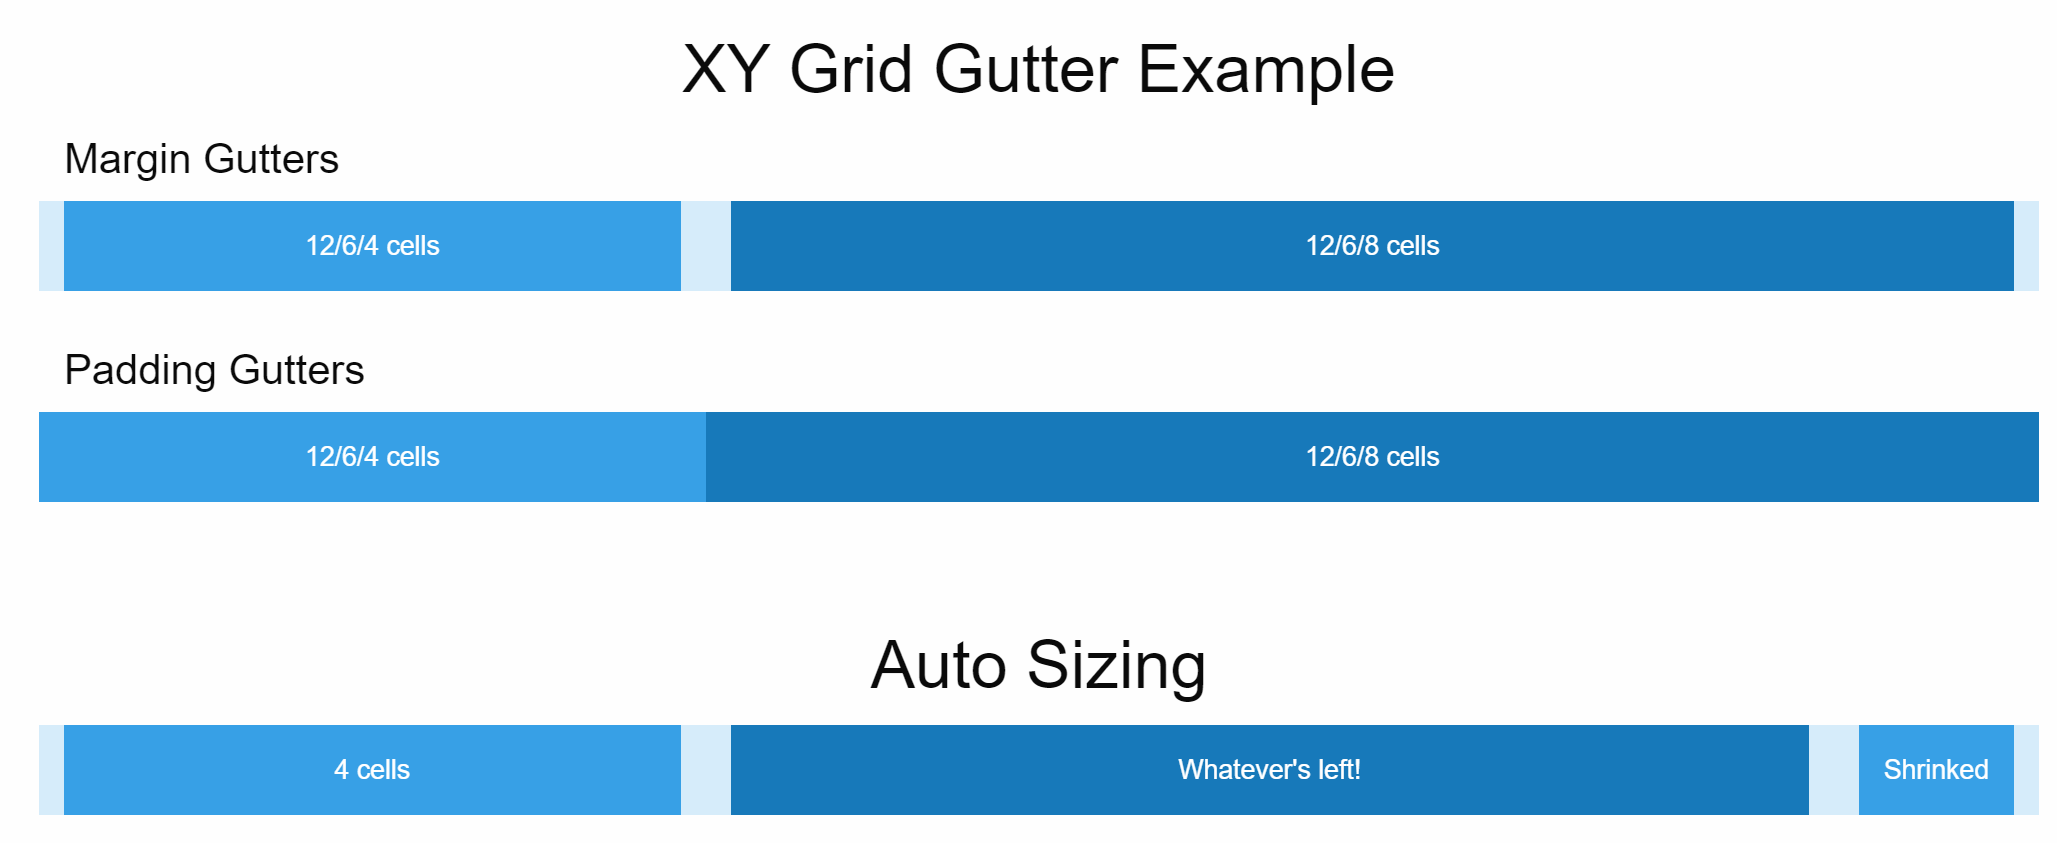
\includegraphics[width=\textwidth,height=\textheight,keepaspectratio]{analisis/grid2_f.png}
	\caption{XY grid gutter pada Foundation 6.}
	\label{fig:grid2f}
\end{figure}
Pada gambar ~\ref{fig:grid2f} lebar fitur ditentukan dari XY grid gutter dengan mengggunakan margin dan grid padding secara seimbang. Selain itu fitur auto sizing memungkinkan lebar cell yang tidak didefinisikan dapat menyesuaikan lebarnya dengan keseluuruhan cell yang terbentuk sebelumnya.
\begin{figure} [H]
	\centering  
	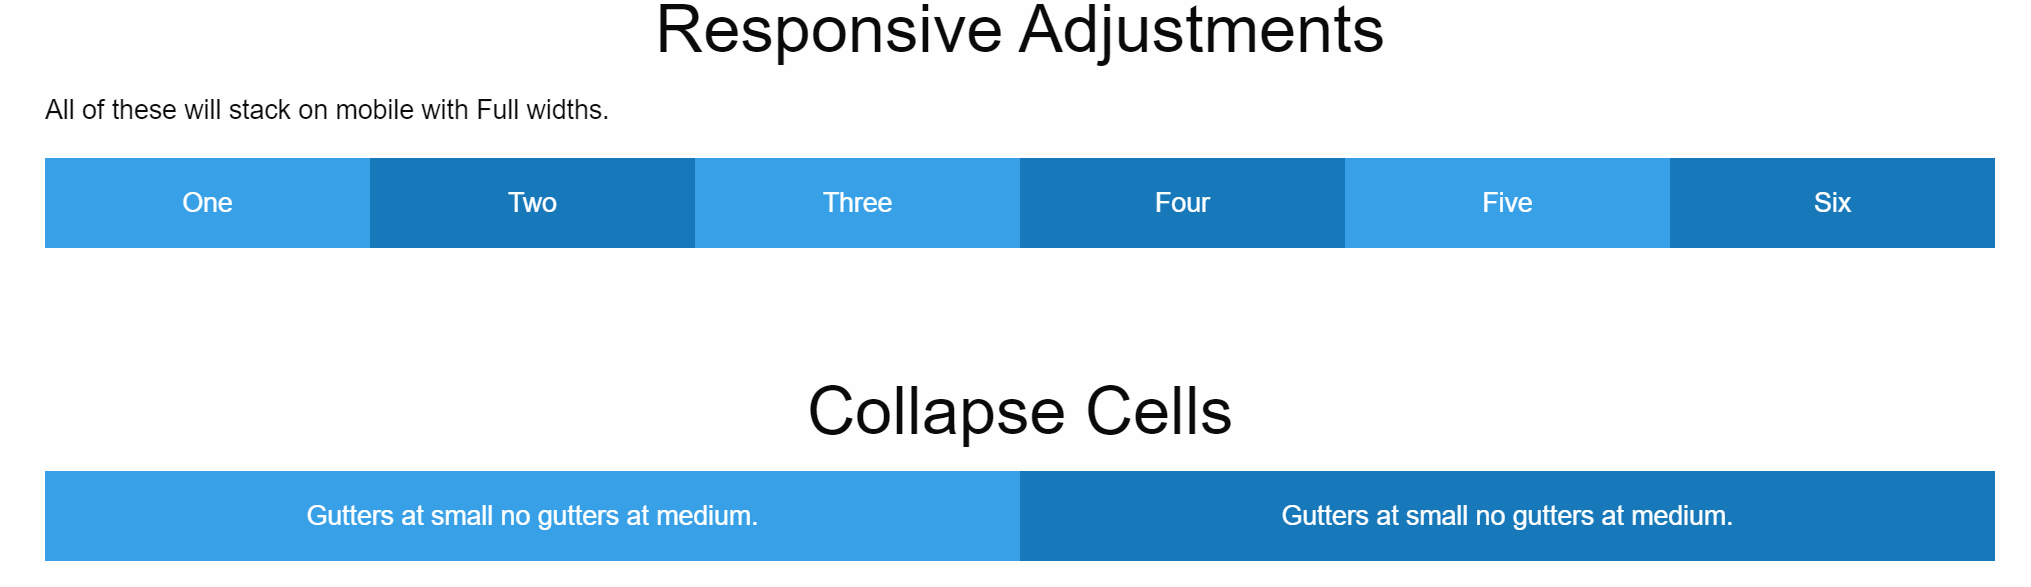
\includegraphics[width=\textwidth,height=\textheight,keepaspectratio]{analisis/grid3_f.png}
	\caption{Grid 3 pada Foundation 6.}
	\label{fig:grid3f}
\end{figure}
Pada gambar ~\ref{fig:grid3f} \textit{responsive adjustment} berarti sel-sel menumpuk di layar kecil, sksn berubah dan memiliki lebar yang sama pada layar besar. Lalu \textit{collapse cells} memungkinkan untuk menghapus \textit{gutter} yang ada pada cell.

\subsubsection{Bootstrap 4: Flex Grid}
Bootstrap menggunakan sistem grid flex yang memungkinkan untuk membuat layout dengan ukuran yang beragam dengan memanfaatkan sistem kolom 12-grid.\\
\begin{figure} [H]
	\centering  
	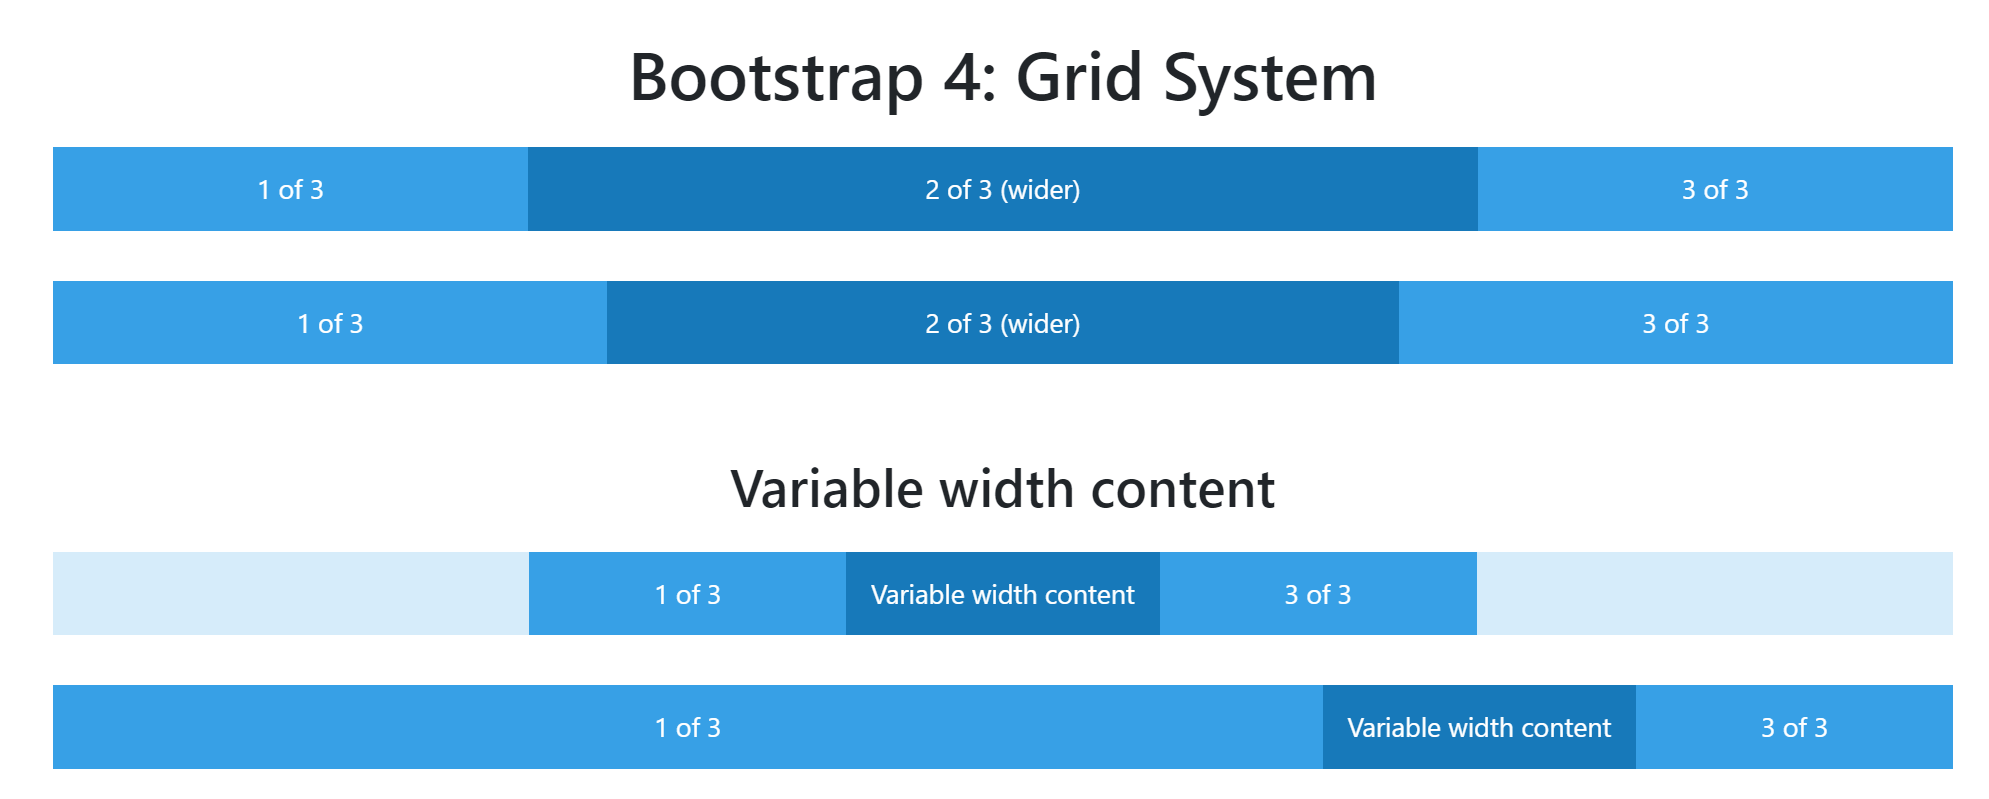
\includegraphics[width=\textwidth,height=\textheight,keepaspectratio]{analisis/grid1_b.png}
	\caption{Grid 1 pada Bootstrap 4.}
	\label{fig:grid1b}
\end{figure}
Pada gambar ~\ref{fig:grid1b} \textit{variable width content} memungkinkan untuk mengukur kolom berdasarkan lebar asli konten .
\begin{figure} [H]
	\centering  
	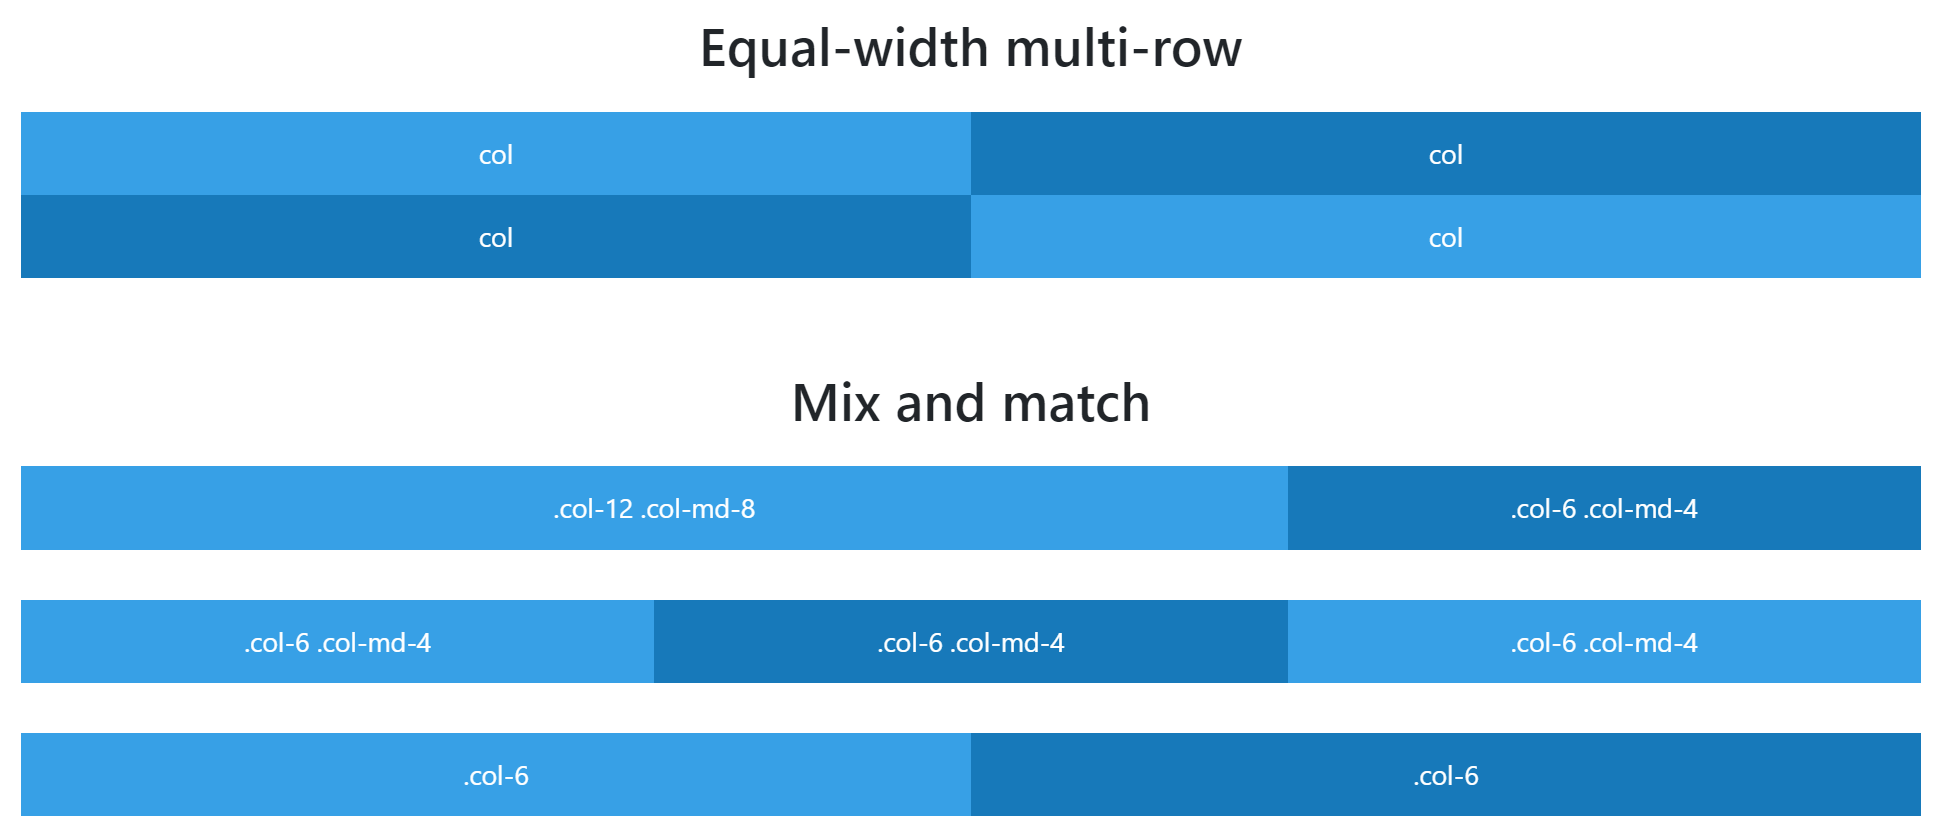
\includegraphics[width=\textwidth,height=\textheight,keepaspectratio]{analisis/grid2_b.png}
	\caption{\textit{variable width content} pada Bootstarp 4.}
	\label{fig:grid2b}V\end{figure}
Pada gambar ~\ref{fig:grid2b} \textit{Equal width multi row } memungkinkan kelas tanpa lebar grid pada setiap kolom akan memiliki lebar yang sama. Sedangkan \textit{mix and match} memungkinkan untuk menggabugkan lebih dari satu kelas dalam satu cell.
\begin{figure} [H]
	\centering  
	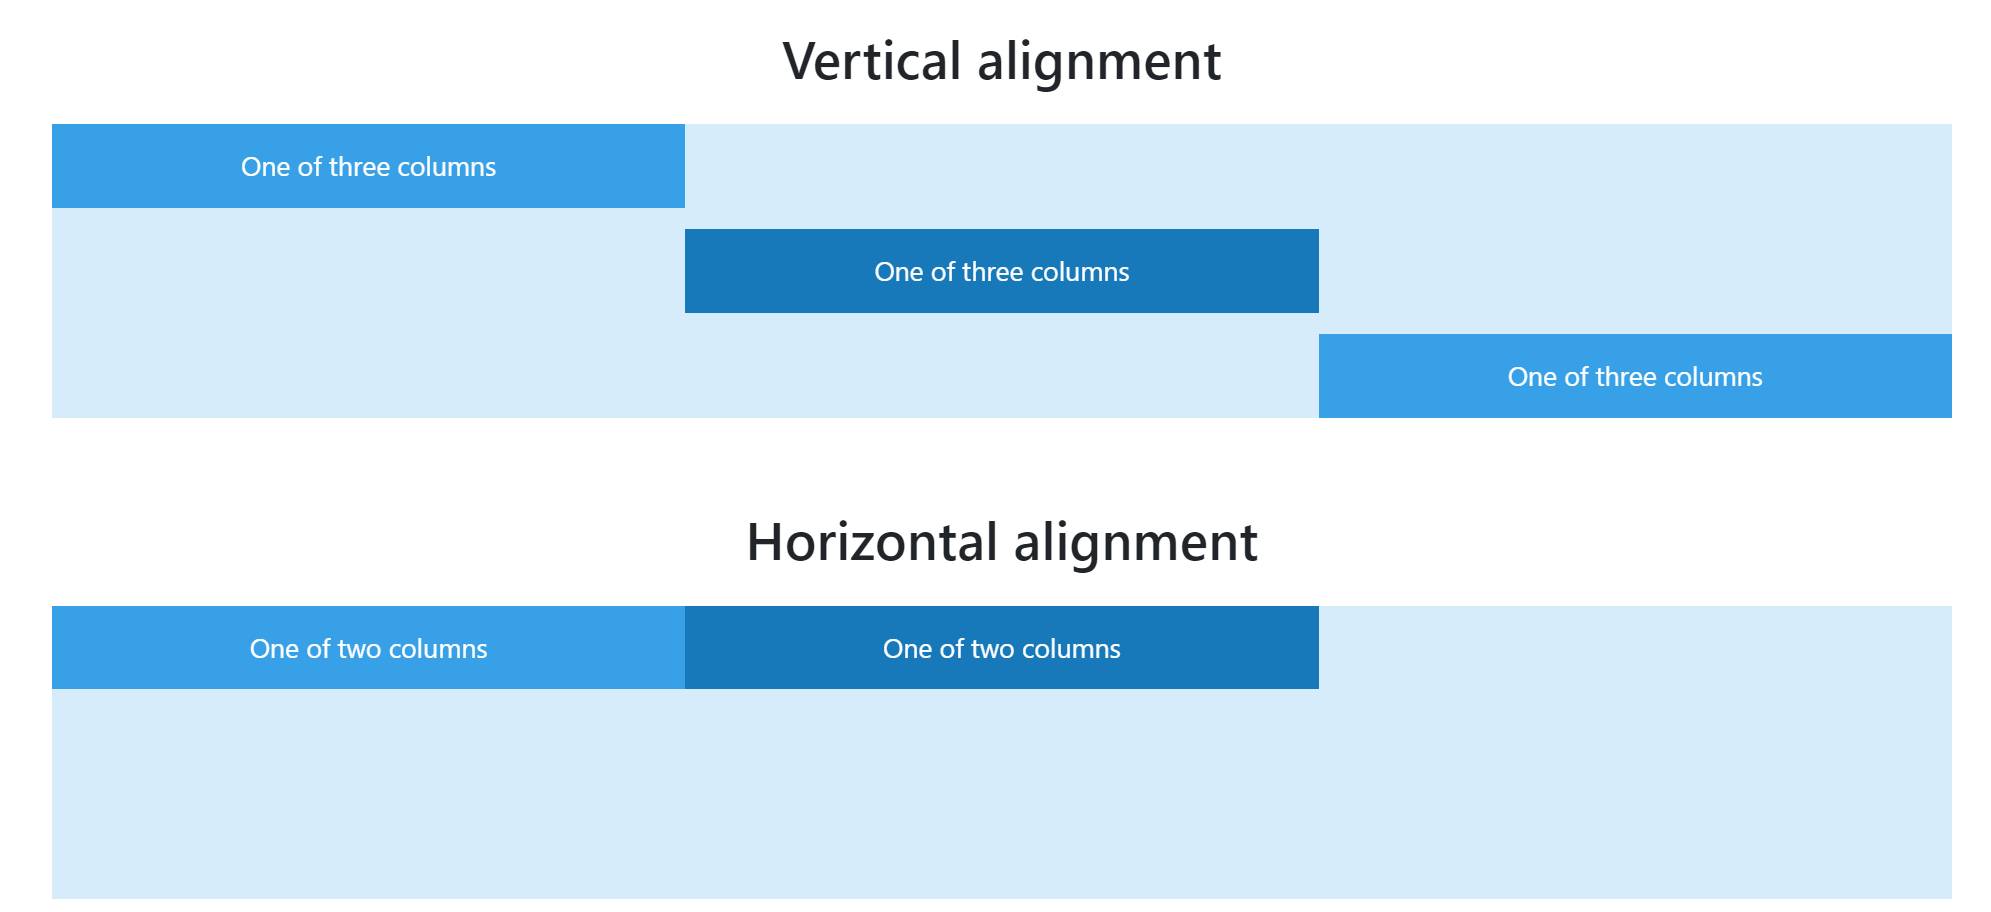
\includegraphics[width=\textwidth,height=\textheight,keepaspectratio]{analisis/grid3_b.png}
	\caption{Grid 3 pada Bootstarp 4.}
	\label{fig:grid3b}
\end{figure}
Pada gambar ~\ref{fig:grid3b} memungkinkan penggunaan flexbox untuk meluruskan kolom secara vertikal dan horizontal.

\section{Navigation}
\subsubsection{Foundation 6: Navigation}
Berikut ini visualisasi komponen menu navigasi di Foundation 6 terlihat pada gambar ~\ref{fig:menuFoundation}:
\begin{figure} [H]
	\centering  
	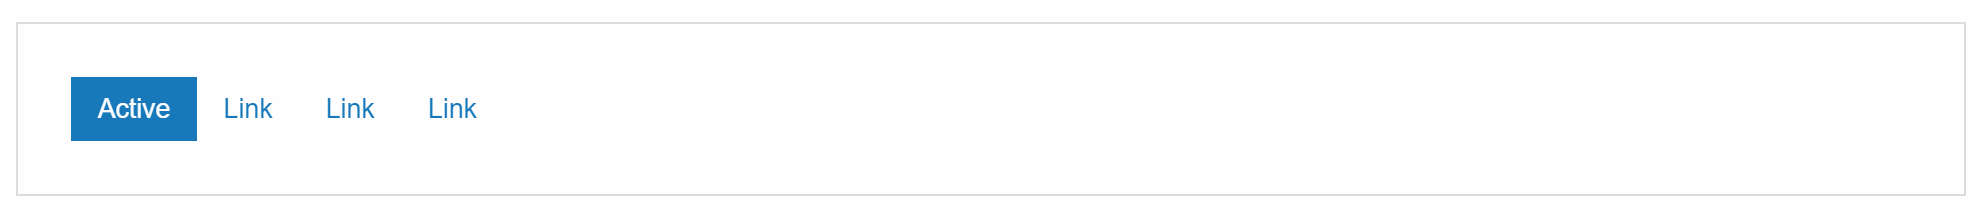
\includegraphics[scale=0.7]{analisis/menu_foundation.png}  
	\caption{Menu pada Foundation 6.}
	\label{fig:menuFoundation}	 
\end{figure}

\subsubsection{Bootstrap 4: Navbar}
Berikut ini visualisasi komponen menu navigasi di Bootstrap 4 terlihat pada gambar ~\ref{fig:menuBootstrap}:
\begin{figure} [H]
	\centering  
	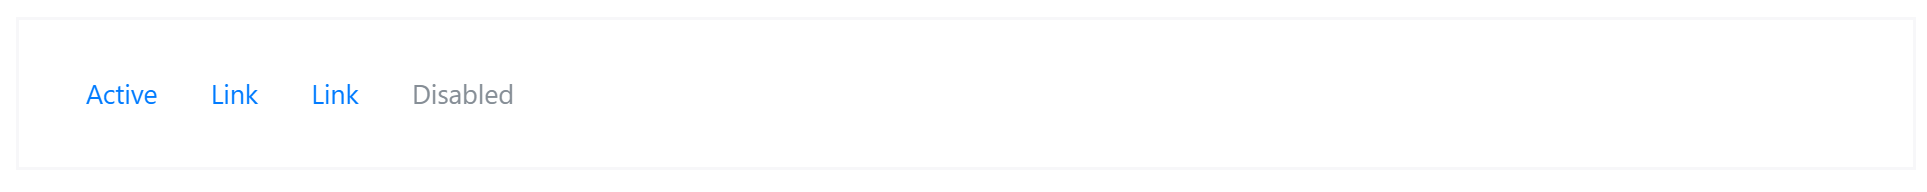
\includegraphics[scale=0.7]{analisis/menu_bootstrap.png}  
	\caption{Menu pada Bootstrap 4.}
	\label{fig:menuBootstrap}	 
\end{figure}

\subsubsection{Perbedaan penggunaan kelas}
\noindent Perbandingan penggunaan kelas pada Foundation 6 (Gambar ~\ref{fig:menuFoundation}) dan Bootstrap 4 (Gambar ~\ref{fig:menuBootstrap}) pada menu navigasi tertera pada tabel ~\ref{table:konversiNavigasi}.\\
\begin{table}[H]
	\caption{Tabel menu navigasi pada Foundation 6 dan Bootstrap 4.}
	\begin{tabular}{| p{0.35\textwidth} | p{0.27\textwidth} | p{0.27\textwidth} |} 
		\hline
		\textbf{Jenis Komponen} & \textbf{Foundation 6} & \textbf{Bootstrap 4}  \\ [0.5ex] 
		\hline	
		Menu &\texttt{.menu} & \texttt{.nav } \\
		\hline	
		Daftar submenu & - & \texttt{.nav-item} \\
		\hline
		Link submenu & - & \texttt{.nav-link} \\
		\hline
		Submenu aktif & \texttt{.is-active} & \texttt{.active}  \\
		\hline
		Sub-menu disabled & - & \texttt{nav-link disabled}  \\[1ex] 
		\hline
	\end{tabular}
	\label{table:konversiNavigasi}
\end{table}
Pemberian kelas pada daftar submenu dan link tidak terjadi pada Foundation 6, hanya menggunakan kode HTML \texttt{<li>} dan \texttt{<a>}.

\section{Form}
\subsubsection{Foundation 6: Forms}
Berikut ini visualisasi komponen forms di Foundation 6 terlihat pada gambar ~\ref{fig:formFoundation}:
\begin{figure} [H]
	\centering  
	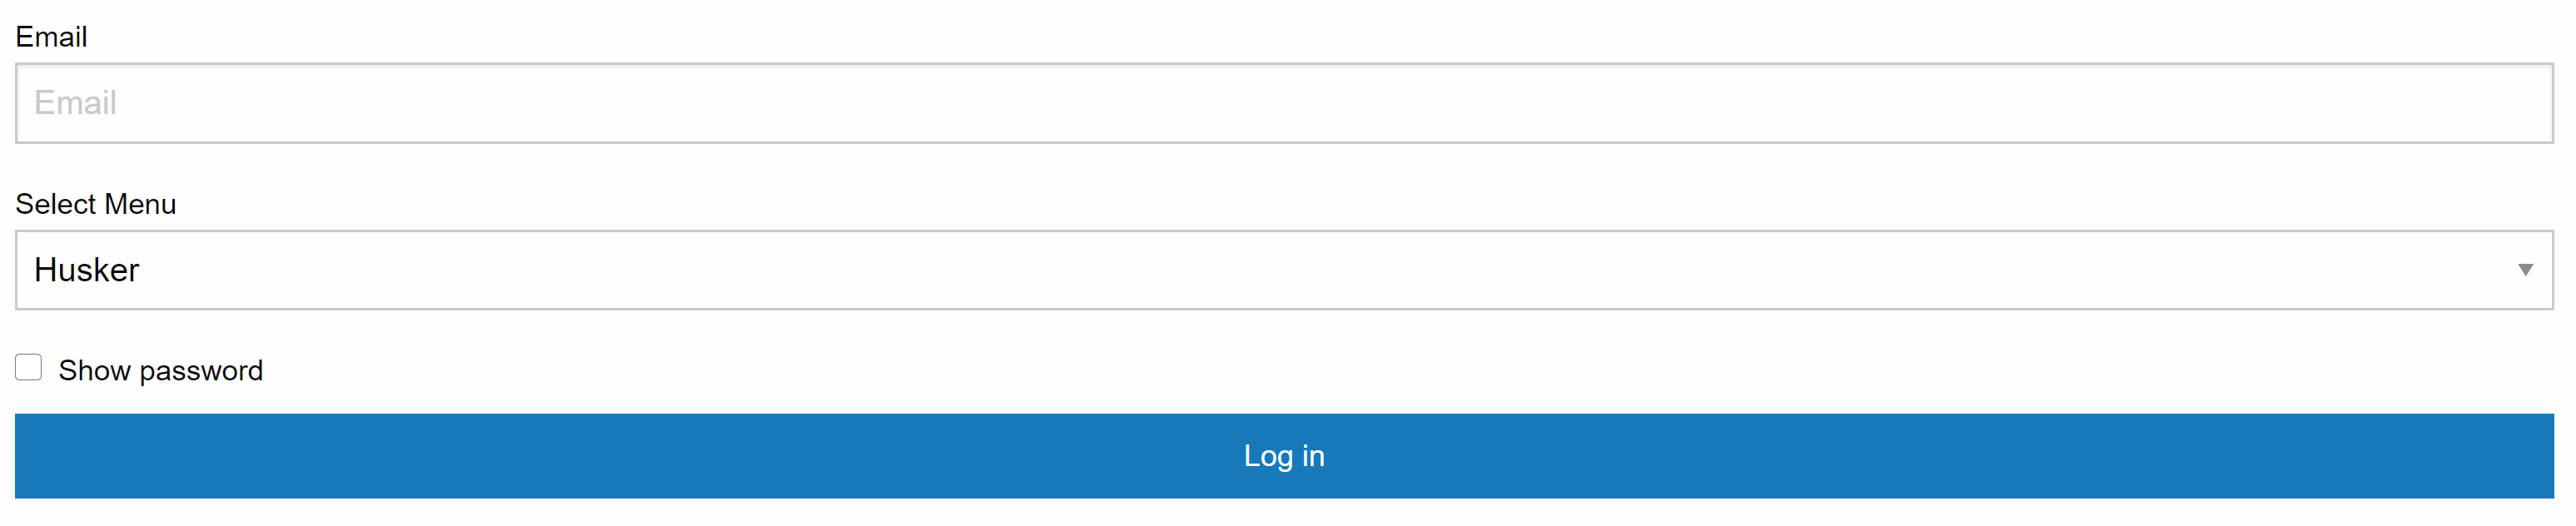
\includegraphics[width=\textwidth,height=\textheight,keepaspectratio]{analisis/form_foundation.png}  
	\caption{\textit{Forms} pada Foundation 6.}
	\label{fig:formFoundation}	 
\end{figure}


\subsubsection{Bootstrap 4: Forms}
Berikut ini visualisasi komponen forms di Bootstrap 4 terlihat pada gambar ~\ref{fig:formBootstrap}:
\begin{figure} [H]
	\centering  
	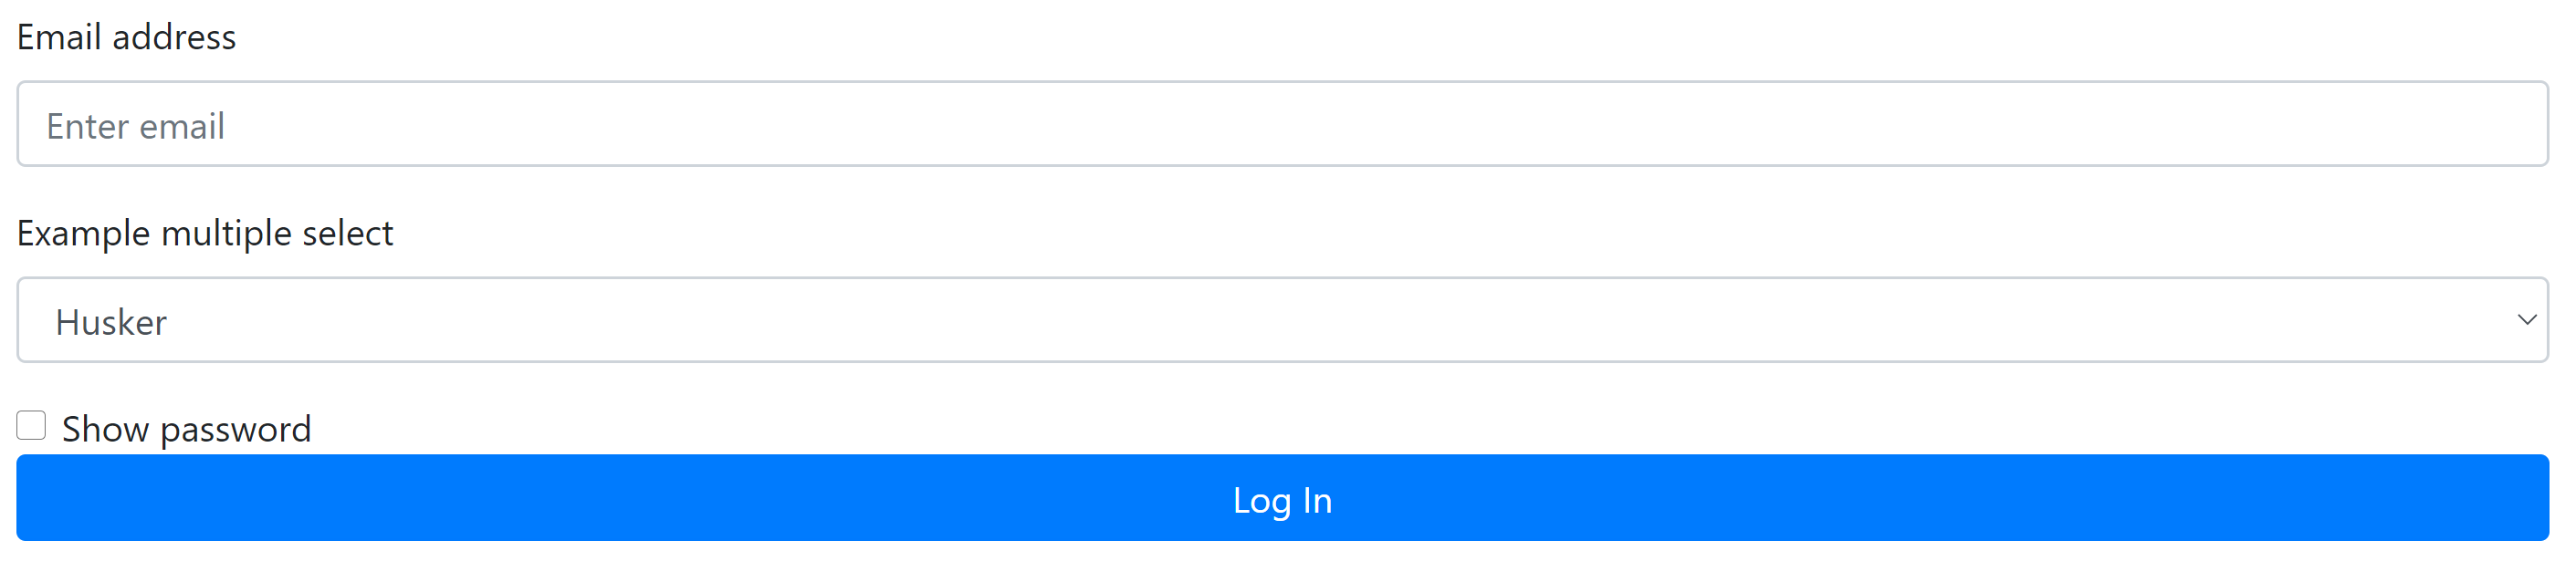
\includegraphics[width=\textwidth,height=\textheight,keepaspectratio]{analisis/form_bootstrap.png}  
	\caption{\textit{Forms} pada Bootstrap 4.}
	\label{fig:formBootstrap}	 
\end{figure}

\subsubsection{Perbedaan penggunaan kelas}
\noindent Perbandingan penggunaan kelas pada Foundation 6 (Gambar ~\ref{fig:formFoundation}) dan Bootstrap 4 (Gambar ~\ref{fig:formBootstrap}) pada menu navigasi tertera pada tabel ~\ref{table:form}.\\

\begin{table}[H] 
	\caption{Kelas form pada Foundation 6 dan Bootstrap 4.}
	\begin{tabular}{| p{0.35\textwidth} | p{0.27\textwidth} | p{0.27\textwidth} |} 
		\hline
		\textbf{Jenis Komponen} & \textbf{Foundation 6} & \textbf{Bootstrap 4}  \\ [0.5ex] 
		\hline	
		\textit{Form group} & - & \texttt{.form-group}\\
		\hline
		\textit{Input} & - & \texttt{.form-control}\\
		\hline			
		Tombol berwarna biru & \texttt{.button} & \texttt{.btn-primary}  \\
		\hline
		Tombol \textit{expand} & \texttt{.alert button} & \texttt{.btn btn-danger} \\[1ex]
		\hline
	\end{tabular}
	\label{table:form}
\end{table}

\section{Inline Labels and Buttons}
\subsubsection{Foundation 6: Inline Labels and Buttons}
Berikut ini visualisasi komponen \textit{inline labels} dan \textit{buttons} di Foundation 6 terlihat pada gambar ~\ref{fig:inlineFoundation}:
\begin{figure} [H]
	\centering  
	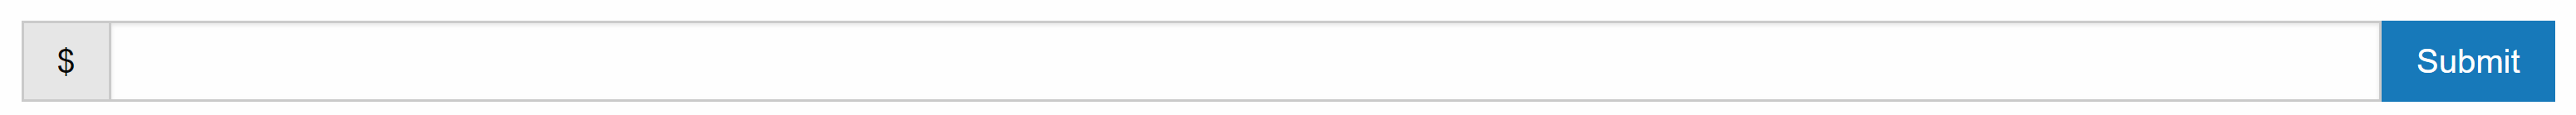
\includegraphics[width=\textwidth,height=\textheight,keepaspectratio]{analisis/inline_foundation.png}  
	\caption{\textit{Inline forms} pada Foundation 6.}
	\label{fig:inlineFoundation}	 
\end{figure}

\subsubsection{Bootstrap 4: Input Groups}
Berikut ini visualisasi komponen \textit{input groups} di Bootstrap 4 terlihat pada gambar ~\ref{fig:inlineBootstrap}:
\begin{figure} [H]
	\centering  
	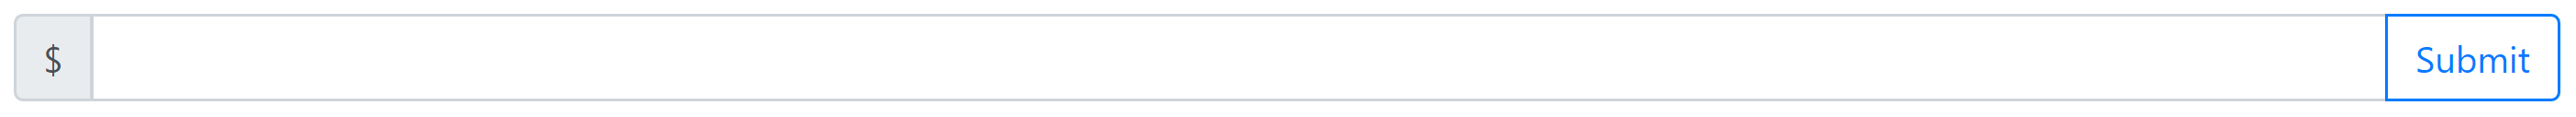
\includegraphics[width=\textwidth,height=\textheight,keepaspectratio]{analisis/inline_bootstrap.png}  
	\caption{\textit{Inline forms} pada Bootstrap 4.}
	\label{fig:inlineBootstrap}	 
\end{figure}

\subsubsection{Perbedaan penggunaan kelas}
\noindent Perbandingan penggunaan kelas pada Foundation 6 (Gambar ~\ref{fig:inlineFoundation}) dan Bootstrap 4 (Gambar ~\ref{fig:inlineBootstrap}) pada menu navigasi tertera pada tabel ~\ref{table:inlineForm}.\\

\begin{table}[H] 
	\caption{Kelas inline form pada Foundation 6 dan Bootstrap 4.}
	\begin{tabular}{| p{0.35\textwidth} | p{0.27\textwidth} | p{0.27\textwidth} |} 
		\hline
		\textbf{Jenis Komponen} & \textbf{Foundation 6} & \textbf{Bootstrap 4}  \\ [0.5ex] 
		\hline	
		\textit{Form group} & \texttt{.input-group} & \texttt{.input-group}\\
		\hline
		Elemen didepan input & - & \texttt{.input-group-prepend}\\
		\hline
		Elemen dibelakang input & - & \texttt{.input-group-append}\\
		\hline
		Input group label & \texttt{input-group-label} & \texttt{.input-group-text}\\
		\hline
		Input group field & \texttt{input-group-field} & - \\
		\hline
		Input group button & \texttt{input-group-button} & -\\
		\hline
		\textit{Input} & - & \texttt{.form-control}\\ [1ex]
		\hline
	\end{tabular}
	\label{table:inlineForm}
\end{table}

\section{Button}
\subsubsection{Foundation 6: Button}
Berikut ini visualisasi komponen \textit{button}di Foundation 6 terlihat pada gambar ~\ref{fig:buttonFoundation}:
\begin{figure} [H]	
	\centering
	
\includegraphics[scale=0.7]{analisis/button_foundation.png}
	\caption{Komponen button Foundation 6.}
	\label{fig:buttonFoundation}
\end{figure}

\subsubsection{Bootstrap 4: Button}
Berikut ini visualisasi komponen \textit{button} di Bootstrap 4 terlihat pada gambar ~\ref{fig:buttonBootstrap}:
\begin{figure} [H]	
	\centering
	
\includegraphics[scale=0.7]{analisis/button_bootstrap.png}
	\caption{Komponen button Bootstrap 4.}
	\label{fig:buttonBootstrap}
\end{figure}

\subsubsection{Perbedaan penggunaan kelas}
\noindent Perbandingan penggunaan kelas pada Foundation 6 (gambar ~\ref{fig:buttonFoundation}) dan Bootstrap 4 (gambar ~\ref{fig:buttonBootstrap}) pada komponen button tertera pada tabel ~\ref{table:button}.\\

\begin{table}[H] 
	\caption{Kelas \textit{button} pada Foundation 6 dan Bootstrap 4.}
	\begin{tabular}{| p{0.35\textwidth} | p{0.27\textwidth} | p{0.27\textwidth} |} 
		\hline
		\textbf{Jenis Komponen} & \textbf{Foundation 6} & \textbf{Bootstrap 4}  \\ [0.5ex] 
		\hline	
		\textit{Button} berwarna hijau & \texttt{.success button} & \texttt{.btn btn-success}\\ 
		\hline
		\textit{Button} berwarna merah & \texttt{.danger button} & \texttt{.btn btn-danger}\\ [1ex]
		\hline
	\end{tabular}
	\label{table:button}
\end{table}

\section{Label}	
\subsubsection{Foundation 6: Label}
Berikut ini visualisasi komponen label di Foundation 6 terlihat pada gambar ~\ref{fig:labelFoundation}:
	\begin{figure}[H]
		\centering  
		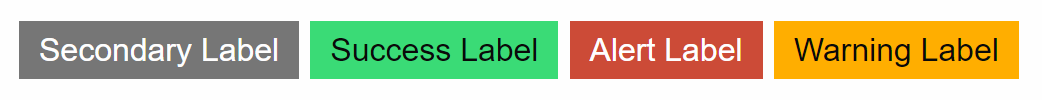
\includegraphics[width=\textwidth,height=\textheight,keepaspectratio]{analisis/label_foundation.png}
		\caption{Foundation 6.} 
		\label{fig:labelFoundation}
	\end{figure}
\subsubsection{Bootstrap 4: Badges}
Berikut ini visualisasi komponen \textit{badges} di Bootstrap 4 terlihat pada gambar ~\ref{fig:labelBootstrap}:
	\begin{figure}[H] 
		\centering
		
\includegraphics[width=\textwidth,height=\textheight,keepaspectratio]{analisis/label_bootstrap.png}
		\caption{Bootstrap 4.} 
		\label{fig:labelBootstrap}
	\end{figure}
	

\subsubsection{Perbedaan penggunaan kelas}
\noindent Perbandingan penggunaan kelas pada Foundation 6 (gambar ~\ref{fig:labelFoundation}) dan Bootstrap 4 (gambar ~\ref{fig:labelBootstrap}) pada komponen label tertera pada tabel ~\ref{table:label}.\\

\begin{table}[H] 
	\caption{Kelas label pada Foundation 6 dan Bootstrap 4.}
	\begin{tabular}{| p{0.35\textwidth} | p{0.27\textwidth} | p{0.27\textwidth} |} 
		\hline
		\textbf{Jenis Komponen} & \textbf{Foundation 6} & \textbf{Bootstrap 4}  \\ [0.5ex] 
		\hline	
		Label berwarna abu & \texttt{.label secondary} & \texttt{.badge badge-secondary}\\ 
		\hline
		Label berwarna hijau & \texttt{.label success} & \texttt{.badge badge-success}\\ 
		\hline
		Label berwarna merah & \texttt{.label alert} & \texttt{.badge badge-danger}\\ 
		\hline
		Label berwarna kuning & \texttt{.label warning} & \texttt{.badge badge-warning}\\ [1ex]
		\hline
	\end{tabular}
	\label{table:label}
\end{table}

\section{Card}

\subsubsection{Foundation 6: Card}
Berikut ini visualisasi komponen \textit{card} di Foundation 6 terlihat pada gambar ~\ref{fig:cardFoundation}:
\begin{figure} [H]	
	\centering
	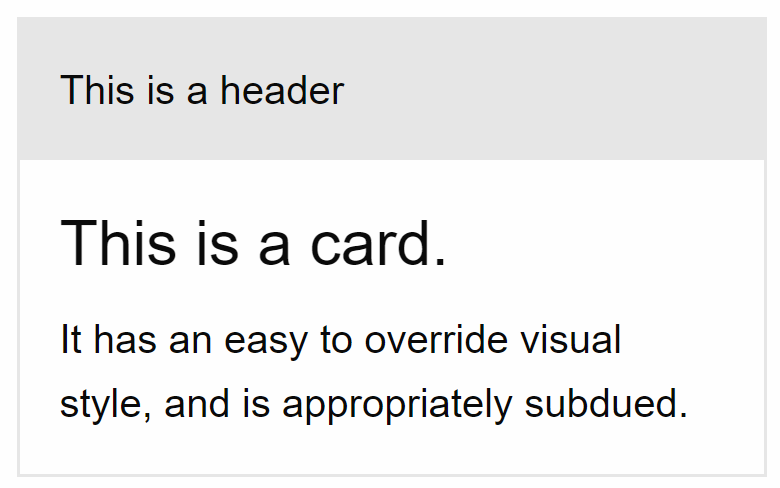
\includegraphics[scale=0.7]{analisis/card_foundation.png}
	\caption{Komponen card pada Foundation 6.}
	\label{fig:cardFoundation}	
\end{figure}

\subsubsection{Bootstrap 4: Card}
Berikut ini visualisasi komponen \textit{card} di Bootstrap 4 terlihat pada gambar ~\ref{fig:cardBootstrap}:
\begin{figure} [H]
	\centering
	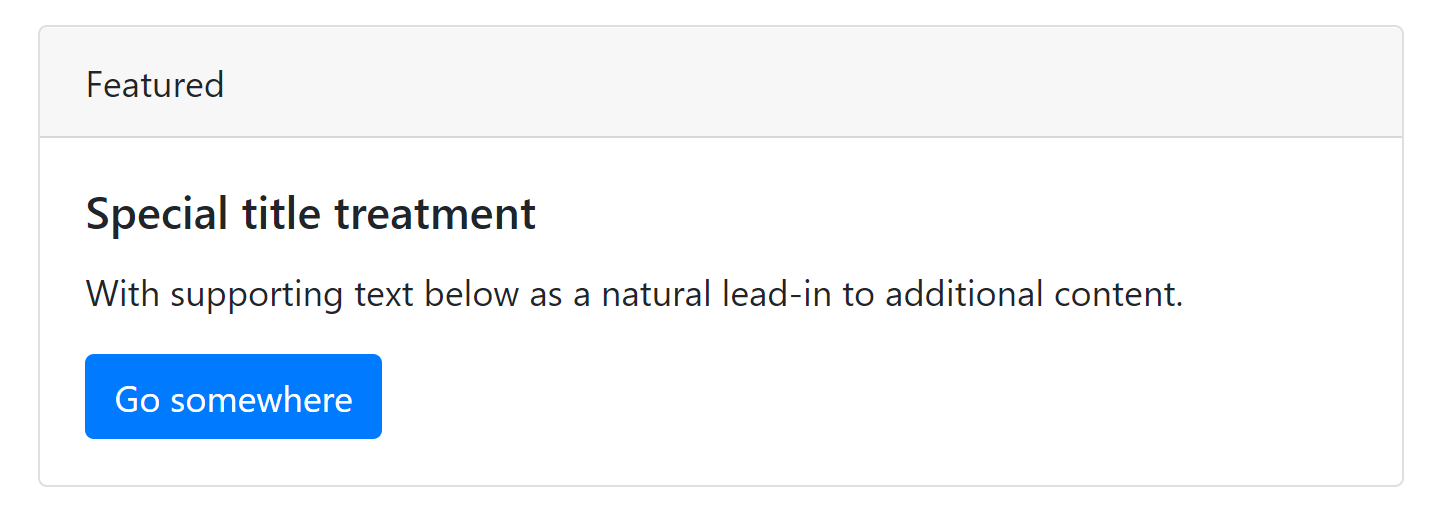
\includegraphics[scale=0.7]{analisis/card_bootstrap.png}
	\caption{Komponen card pada Bootstrap 4.}
	\label{fig:cardBootstrap}
\end{figure}

\subsubsection{Perbedaan penggunaan kelas}
\noindent Perbandingan penggunaan kelas pada Foundation 6 (gambar ~\ref{fig:cardFoundation}) dan Bootstrap 4(gambar ~\ref{fig:cardBootstrap}) pada komponen card tertera pada tabel ~\ref{table:label}.\\

\begin{table}[H] 
	\caption{Kelas label pada Foundation 6 dan Bootstrap 4.}
	\begin{tabular}{| p{0.35\textwidth} | p{0.27\textwidth} | p{0.27\textwidth} |} 
		\hline
		\textbf{Jenis Komponen} & \textbf{Foundation 6} & \textbf{Bootstrap 4}  \\ [0.5ex] 
		\hline	
		Card & \texttt{.card} & \texttt{.card}\\ 
		\hline
		Judul card & \texttt{.card-divider} & \texttt{.card-header}\\ 
		\hline
		Isi card & \texttt{.card-section} & \texttt{.card-body}\\ [1ex]
		\hline
	\end{tabular}
	\label{table:card}
\end{table}

\section{Modal}
\subsubsection{Foundation 6: Modal}
Berikut ini visualisasi komponen \textit{modal} di Foundation 6 terlihat pada gambar ~\ref{fig:modalFoundation}:
\begin{figure} [H]	
	\centering
	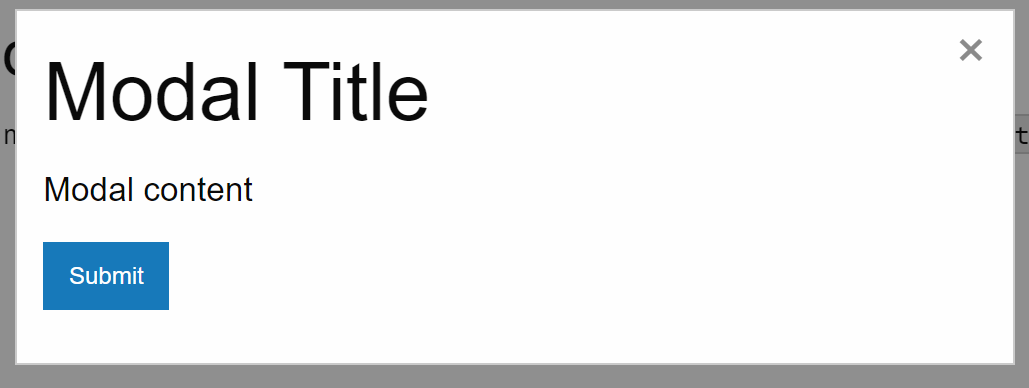
\includegraphics[scale=0.7]{analisis/modal_foundation.png}
	\caption{Komponen modal pada Foundation 6.}
	\label{fig:modalFoundation}
\end{figure}

\subsubsection{Bootstrap 4: Modal}
Berikut ini visualisasi komponen \textit{modal} di Bootstrap 4 terlihat pada gambar ~\ref{fig:modalBootstrap}:
\begin{figure} [H]
	\centering
	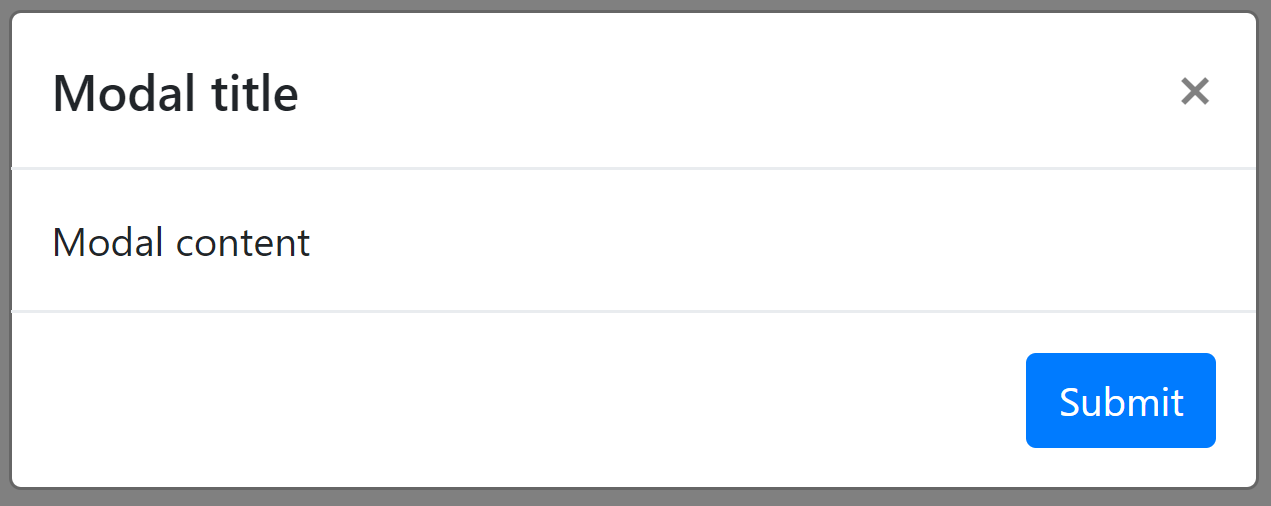
\includegraphics[scale=0.7]{analisis/modal_bootstrap.png}
	\caption{Komponen modal pada Bootstrap 4.}
	\label{fig:modalBootstrap}
\end{figure}

\subsubsection{Perbedaan penggunaan kelas}
\noindent Perbandingan penggunaan kelas pada Foundation 6 (gambar ~\ref{fig:modalFoundation}) dan Bootstrap 4 (gambar ~\ref{fig:modalBootstrap}) pada komponen modal tertera pada tabel ~\ref{table:modal}.\\


\begin{table}[H] 
	\caption{Kelas modal pada Foundation 6 dan Bootstrap 4.}
	\begin{tabular}{| p{0.35\textwidth} | p{0.27\textwidth} | p{0.27\textwidth} |} 
		\hline
		\textbf{Jenis Komponen} & \textbf{Foundation 6} & \textbf{Bootstrap 4}  \\ [0.5ex] 
		\hline	
		Modal & \texttt{.reveal} & \texttt{.modal fade}\\ 
		&\texttt{data-reveal}&\texttt{.modal-dialog}\\
		&&\texttt{.modal-content}\\
		\hline
		Link & \texttt{data-open} & \texttt{data-toggle}\\
		&& \texttt{data-target}\\
		\hline
		Header & - & \texttt{.modal-header}\\ 
		\hline
		Judul modal & - & \texttt{.modal-title}\\ 
		\hline
		Isi modal & - & \texttt{.modal-body}\\ 
		\hline
		\texttt{Footer} & - & \texttt{.modal-footer}\\
		\hline
		\texttt{Close} & \texttt{.close button} & \texttt{.close}\\
		& \texttt{data-close} & \texttt{data-dismiss}\\
		& \texttt{aria-label}&\\[1ex]
		\hline
	\end{tabular}
	\label{table:modal}
\end{table}

\section{Table}
\subsubsection{Foundation 6: Table}
Berikut ini visualisasi komponen \textit{table} di Foundation 6 terlihat pada gambar ~\ref{fig:tabelFoundation}:
\begin{figure} [H]	
	\centering
	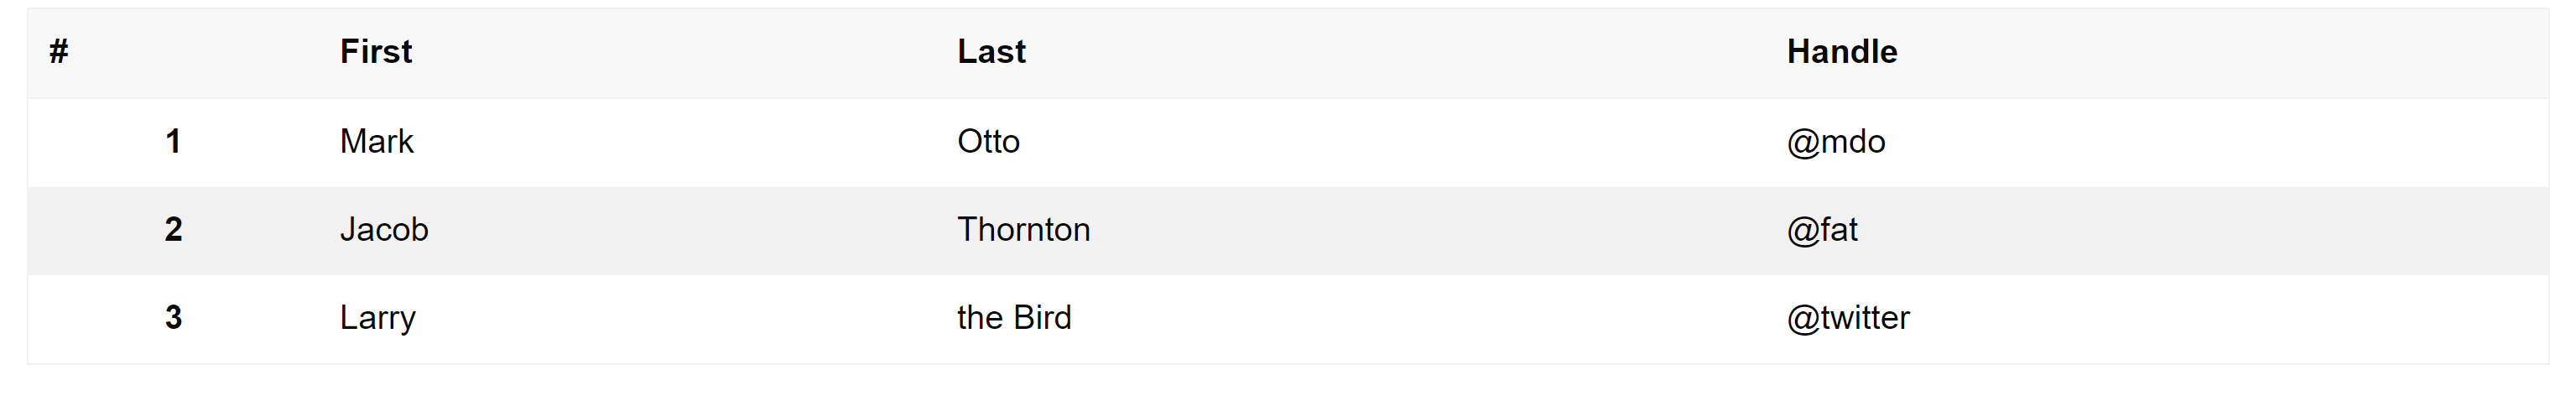
\includegraphics[width=\textwidth,height=\textheight,keepaspectratio]{analisis/table_foundation.png}
	\caption{Komponen tabel pada Foundation 6.}
	\label{fig:tabelFoundation}
\end{figure}

\subsubsection{Bootstrap 4: Table}
Berikut ini visualisasi komponen \textit{table} di Bootstrap 4 terlihat pada gambar ~\ref{fig:tabelBootstrap}:
\begin{figure} [H]
	\centering
	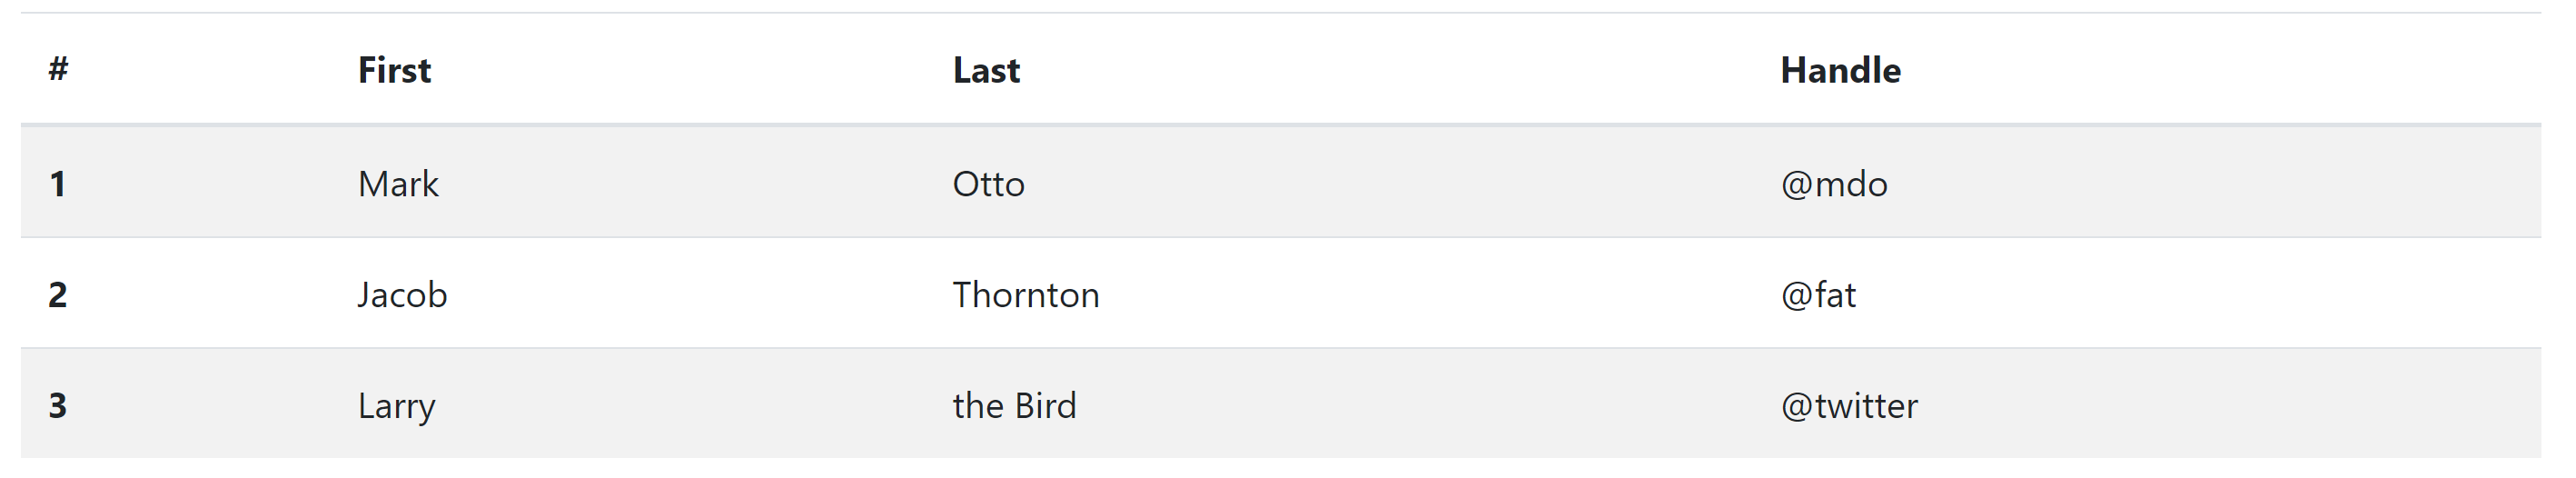
\includegraphics[width=\textwidth,height=\textheight,keepaspectratio]{analisis/table_bootstrap.png}
	\caption{Komponen tabel pada Bootstrap 4.}
	\label{fig:tabelBootstrap}
\end{figure}

\subsubsection{Perbedaan penggunaan kelas}
\noindent Perbandingan penggunaan kelas pada Foundation 6 (gambar ~\ref{fig:tabelFoundation}) dan Bootstrap 4 di gambar ~\ref{fig:tabelBootstrap} pada komponen tabel tertera pada tabel ~\ref{table:tabel}.\\

\begin{table}[H] 
	\caption{Kelas modal pada Foundation 6 dan Bootstrap 4.}
	\begin{tabular}{| p{0.35\textwidth} | p{0.27\textwidth} | p{0.27\textwidth} |} 
		\hline
		\textbf{Jenis Komponen} & \textbf{Foundation 6} & \textbf{Bootstrap 4}  \\ [0.5ex] 
		\hline	
		Tabel & - & \texttt{.table striped}\\[1ex]	
		\hline		
	\end{tabular}
	\label{table:tabel}
\end{table}

\section{Tabs}
\subsubsection{Foundation 6: Tabs}
Berikut ini visualisasi komponen \textit{tabs} di Foundation 6 terlihat pada gambar ~\ref{fig:tabsFoundation}:
\begin{figure} [H]	
	\centering
	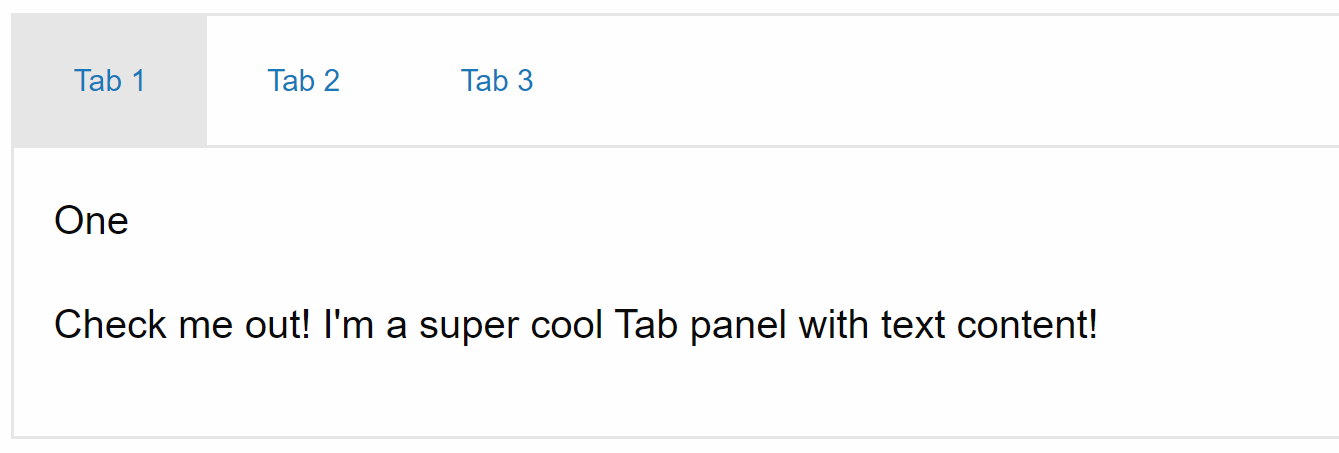
\includegraphics[width=\textwidth,height=\textheight,keepaspectratio]{analisis/tabs_foundation.png}
	\caption{Komponen tabs pada Foundation 6.}
	\label{fig:tabsFoundation}
\end{figure}

\subsubsection{Bootstrap 4: Tabs}
Berikut ini visualisasi komponen \textit{tabs} di Bootstrap 4 terlihat pada gambar ~\ref{fig:tabsBootstrap}:
\begin{figure} [H]
	\centering
	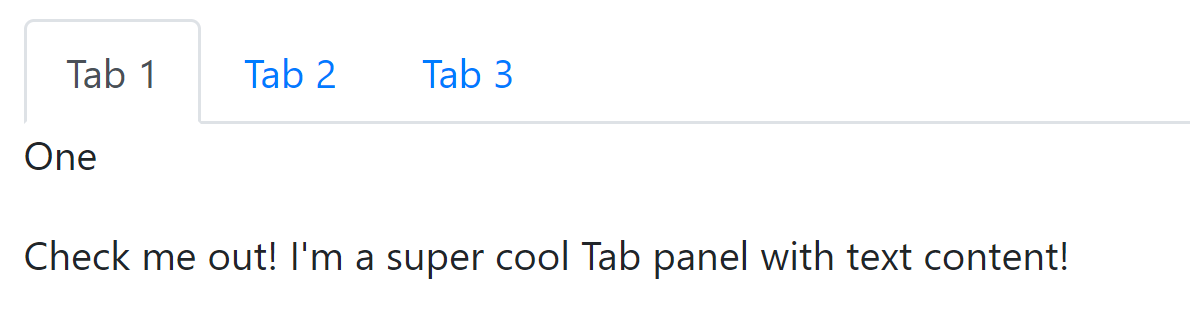
\includegraphics[width=\textwidth,height=\textheight,keepaspectratio]{analisis/tabs_bootstrap.png}
	\caption{Komponen tabs pada Bootstrap 4.}
	\label{fig:tabsBootstrap}
\end{figure}

\subsubsection{Perbedaan penggunaan kelas}
\noindent Perbandingan penggunaan kelas pada Foundation 6 (gambar ~\ref{fig:tabsFoundation}) dan Bootstrap 4  (gambar ~\ref{fig:tabsBootstrap}) pada komponen modal tertera pada tabel ~\ref{table:tabs}.\\

\begin{table}[H] 
	\caption{Kelas modal pada Foundation 6 dan Bootstrap 4.}
	\begin{tabular}{| p{0.35\textwidth} | p{0.27\textwidth} | p{0.27\textwidth} |} 
		\hline
		\textbf{Jenis Komponen} & \textbf{Foundation 6} & \textbf{Bootstrap 4}  \\ [0.5ex] 
		\hline	
		Tabs & \texttt{.tabs} & \texttt{.nav nav-tabs}\\	
		\hline
		Tabs list & \texttt{.tabs-title} & \texttt{.nav nav-item}\\	
		\hline
		Tabs link & - & \texttt{.nav nav-link}\\[1ex]	
		\hline	
		Tabs content & \texttt{.tabs-content} & \texttt{.tab-content}\\[1ex]	
		\hline			
		Tabs panel & \texttt{.tabs-panel} & \texttt{.tab-pane fade}\\[1ex]	
		\hline
		Active tabs panel & \texttt{.is-active} & \texttt{.show active}\\[1ex]	
		\hline	
	\end{tabular}
	\label{table:tabs}
\end{table}

 
